\documentclass[12pt,letterpaper]{article}
\usepackage[utf8]{inputenc}
\usepackage{amsmath}
\usepackage{amsfonts}
\usepackage{amssymb}
\usepackage{amsthm}
\usepackage{graphicx}
\usepackage{tabularx}
\usepackage[left=1cm,right=2cm,top=2cm,bottom=2cm]{geometry}
\usepackage{multicol}
\usepackage{lastpage}
\usepackage{fancyhdr}
\usepackage{multirow,array}
\usepackage{newtxtext,newtxmath}
\usepackage{lastpage}
\usepackage{enumitem}
\newcolumntype{Y}{>{\centering\arraybackslash}X}
\pagestyle{fancy}
\fancyhf{}
\lhead{\textsc{BHCC Mat-181}}
\chead{\textsc{Answers}}
\rhead{\textsc{HW Exercises 2.22-2.26}}
\rfoot{Page \thepage ~of \pageref{LastPage}}
\setenumerate[1]{label={\bf 2.\theenumi: }}
\setenumerate[2]{label={\bf (\theenumii): }}
\setenumerate[3]{label={\bf \theenumiii: }}

\begin{document}
\newcommand{\AND}{\textsc{~and~}}
\newcommand{\OR}{\textsc{~or~}}

\begin{enumerate}
\setcounter{enumi}{21}
\item Let event $S$ represent ``sick'' and $T$ represent ``positive test''.
We are told:
\begin{align*}
P(S) &= 0.03 \\
P(T|S) &= 0.99 \\
P(T^c|S^c) &= 0.98
\end{align*}
We are asked to determine $P(S|T)$. To do so, we can make a tree.
\begin{center}
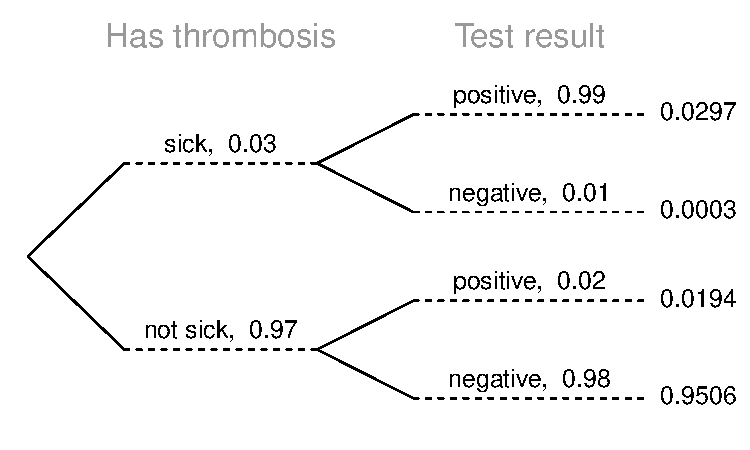
\includegraphics[scale=0.8]{figures/thromb.pdf}
\end{center}
I like to make a contingency table.
\begin{center}
\begin{tabular}{c | c c | c} 
         & pos    & neg    & total \\ \hline
sick     & 0.0297 & 0.0003 & 0.03 \\
not sick & 0.0194 & 0.9506 & 0.97 \\ \hline 
total    & 0.0491 & 0.9509 & 1 
\end{tabular}
\end{center}
Then, it is easy to calculate the conditional probability.
\begin{align*}
P(\text{sick}|\text{pos}) &= \frac{P(\text{sick} \AND \text{pos})}{P(\text{pos})} \\\\
&= \frac{0.0297}{0.0491} \\\\
&\approx \fbox{0.605}
\end{align*}

\newpage
\newcommand{\sick}{\text{sick}}
\newcommand{\nsick}{\text{not sick}}
\newcommand{\pos}{\text{pos}}
\newcommand{\nega}{\text{neg}}
\item We are told:
\begin{align*}
P(\sick) &= 0.259 \\
P(\pos|\sick) &= 0.997 \\
P(\nega|\nsick) &= 0.926
\end{align*}
We are asked to determine $P(\sick|\pos)$. To do so, we can make a tree.
\begin{center}
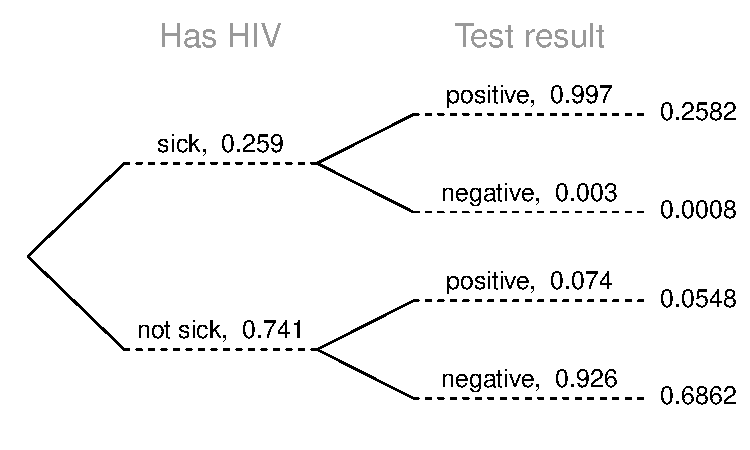
\includegraphics[scale=0.8]{figures/hiv.pdf}
\end{center}
I like to make a contingency table.
\begin{center}
\begin{tabular}{c | c c | c} 
         & pos    & neg    & total \\ \hline
sick     & 0.2582 & 0.0008 & 0.259 \\
not sick & 0.0548 & 0.6862 & 0.741 \\ \hline 
total    & 0.313  & 0.687  & 1 
\end{tabular}
\end{center}
Then, it is easy to calculate the conditional probability.
\begin{align*}
P(\text{sick}|\text{pos}) &= \frac{P(\text{sick} \AND \text{pos})}{P(\text{pos})} \\\\
&= \frac{0.2582}{0.313} \\\\
&\approx \fbox{0.825}
\end{align*}

\newpage

\newcommand{\scott}{\text{scott}}
\newcommand{\nscott}{\text{not scott}}
\newcommand{\college}{\text{college}}
\newcommand{\ncollege}{\text{not college}}
\item We are told:
\begin{align*}
P(\scott) &= 0.53 \\
P(\college|\scott) &= 0.37 \\
P(\college|\nscott) &= 0.44
\end{align*}
We are asked to determine $P(\scott|\college)$. To do so, we can make a tree.
\begin{center}
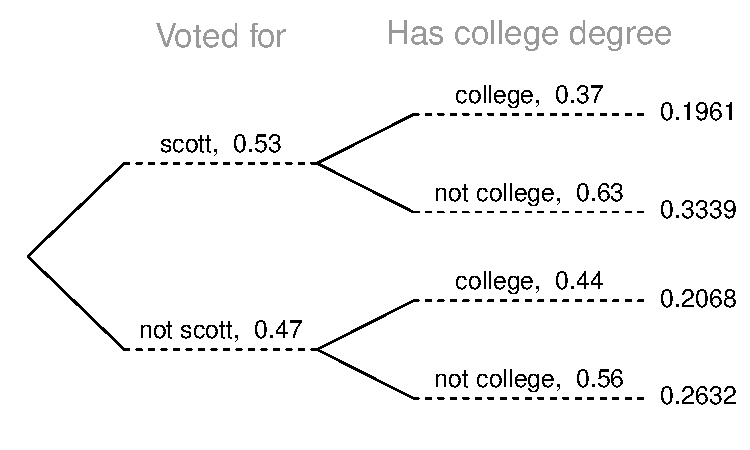
\includegraphics[scale=0.8]{figures/scott.pdf}
\end{center}
I like to make a contingency table.
\begin{center}
\begin{tabular}{c | c c | c} 
         & college& not college    & total \\ \hline
scott    & 0.1961 & 0.3339 & 0.53  \\
not scott& 0.2068 & 0.2632 & 0.47  \\ \hline 
total    & 0.4029 & 0.5971 & 1 
\end{tabular}
\end{center}
Then, it is easy to calculate the conditional probability.
\begin{align*}
P(\text{scott}|\text{college}) &= \frac{P(\text{scott} \AND \text{college})}{P(\text{college})} \\\\
&= \frac{0.1961}{0.0.4029} \\\\
&\approx \fbox{0.825}
\end{align*}

\newpage

\newcommand{\lupus}{\text{lupus}}
\newcommand{\nlupus}{\text{not lupus}}

\item We are told:
\begin{align*}
P(\lupus) &= 0.02 \\
P(\pos|\lupus) &= 0.98 \\
P(\nega|\nlupus) &= 0.74
\end{align*}
We want to determine $P(\lupus|\pos)$. To do so, we could make a tree, but I'll just use the formula.
\begin{align*}
P(\lupus|\pos) &= \cfrac{P(\lupus \AND \pos)}{P(\pos)} \\\\
&= \cfrac{P(\pos|\lupus) \cdot P(\lupus)}{P(\pos|\lupus)\cdot P(\lupus) ~~+~~ P(\pos|\nlupus)\cdot P(\nlupus)}\\\\
&= \cfrac{0.98 \times 0.02}{0.98\times 0.02 ~~+~~ 0.26\times 0.98}\\\\
&= 0.071
\end{align*}
So, even when someone tests positive for lupus, we only think there is about a 7\% chance of them actually having lupus. This kind of supports the notion that often when you think it might be lupus, it actually is not. Of course, about 2\% of the time overall, it really is lupus...

\item We are told that for twins,
\begin{align*}
P(\text{identical}) &= 0.3\\
P(\text{2 girls}|\text{identical}) &= 0.5 \\
P(\text{2 girls}|\text{not identical}) &= 0.25
\end{align*}
We want to determine $P(\text{identical}|\text{2 girls})$. To do so, we could make a tree, but I'll just use the formula.
\begin{align*}
P(\text{identical}|\text{2 girls}) &= \cfrac{P(\text{identical} \AND \text{2 girls})}{P(\text{2 girls})} \\\\
&= \cfrac{P(\text{2 girls} \AND \text{identical})}{P(\text{2 girls} \AND \text{identical}) ~~+~~ P(\text{2 girls}\AND \text{not identical})}\\\\
&= \cfrac{P(\text{2 girls}|\text{identical}) \cdot P(\text{identical})}{P(\text{2 girls}|\text{identical})\cdot P(\text{identical}) ~~+~~ P(\text{2 girls}|\text{not identical})\cdot P(\text{not identical})}\\\\
&= \cfrac{0.5 \times 0.3}{0.5\times 0.3 ~~+~~ 0.25\times 0.7}\\\\
&= \fbox{0.46}
\end{align*}

\end{enumerate}
\end{document}
